% Manual template (AAT2), see docs/HowToDoc.md
% Build (in docs/manual):  pdflatex ManualAmplitudeHistogram.tex   (twice, for the references)
% The PDF is copied into the release zips by the GitHub workflow.
\documentclass[12pt]{article}
\usepackage[utf8]{inputenc}
\usepackage[T1]{fontenc}
\usepackage[top=2cm, bottom=2cm, left=2cm, right=2cm]{geometry}
\usepackage{graphicx}
\usepackage{xcolor}
\usepackage{amsmath}
\usepackage{hyperref}
\hypersetup{colorlinks=true, linkcolor=red, urlcolor=red, pdftitle={AmplitudeHistogram Documentation}}

% ---- change these ------------------------------------------------------------
\newcommand{\pluginversion}{0.2.0}   % the version in CMakeLists.txt
\newcommand{\pluginauthor}{Joerg Bitzer}
\newcommand{\sourceurl}{https://github.com/JoergBitzer/noise_moments}
% -------------------------------------------------------------------------------

\title{AmplitudeHistogram Documentation}
\author{License: CC-BY 4.0}
\date{\today, for AmplitudeHistogram \pluginversion}

\begin{document}
\maketitle

\section{Introduction}
AmplitudeHistogram shows the histogram of the input amplitudes, an estimate of the probability
density function (pdf) of the signal, together with its mean, RMS level, skewness and excess kurtosis.
Over the histogram it draws the normal pdf and the pdf of the Johnson distribution with the measured
skewness and excess kurtosis (the same family its companion plug-in MomentNoise uses to make noise).
Feed it with MomentNoise, and the histogram approaches the theoretical pdf shown by MomentNoise; feed it
with music or speech and see how far real signals are from Gaussian. The audio passes unchanged.

\section{Installation}
The downloaded file is a zip file. It contains the plug-in (.vst3; on macOS also the AU,
.component), the Standalone application, a ReadMeFirst.txt, the licence files and this manual.
Copy the plug-in to the right place and let your DAW rescan its plug-ins.

\begin{verbatim}
Windows (VST3):  C:\Program Files\Common Files\VST3
Mac (VST3):      /Users/yourUSERNAME/Library/Audio/Plug-Ins/VST3
Mac (AU):        /Users/yourUSERNAME/Library/Audio/Plug-Ins/Components
Linux (VST3):    /home/yourUSERNAME/.vst3
\end{verbatim}

The macOS version is not signed with an Apple Developer ID. If macOS reports that the plug-in
is damaged or cannot be opened, remove the quarantine flag in the Terminal, e.g.
\texttt{xattr -cr \textasciitilde/Library/Audio/Plug-Ins/VST3/AmplitudeHistogram.vst3}.

\subsection{Presets and settings}
The presets (plain XML files) and the settings file (\texttt{user.settings}: day/night theme)
are stored in this folder -- delete it to remove AmplitudeHistogram completely:
\begin{verbatim}
Windows: C:\Users\yourUSERNAME\AppData\Roaming\Jade\_Hochschule\AmplitudeHistogram
Mac:     /Users/yourUSERNAME/Library/Audio/Presets/Jade\_Hochschule/AmplitudeHistogram
Linux:   /home/yourUSERNAME/.config/Jade\_Hochschule/AmplitudeHistogram
\end{verbatim}

\section{How to use}
\begin{center}
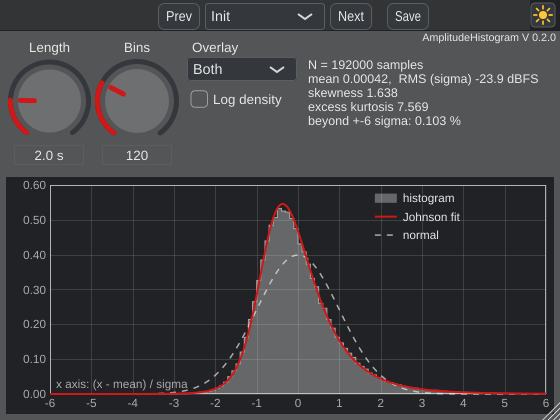
\includegraphics[width=0.8\textwidth]{images/GUI.png}
\end{center}
\begin{enumerate}
    \item \textbf{Preset handler}: Prev/Next step through the presets. To save a new preset,
    type a name and press Save. Save turns red when you change a parameter of the displayed
    preset; press it to update the preset. To delete a preset, delete its XML file.
    \item \textbf{Day/night}: switches between the night (dark) and the day (light) theme.
    \item \textbf{Length} ($0.1 \dots 10$\,s, default 2\,s): the histogram is made of the last samples of
    this duration. All input channels are pooled (stereo: twice the number of samples). Longer means a
    smoother histogram, but a slower reaction to changes.
    \item \textbf{Bins} ($10 \dots 400$, default 120): number of bins between $-6\sigma$ and $6\sigma$.
    The default gives a bin width of $0.1\sigma$: with 2\,s of stereo audio at 48\,kHz (192\,000 samples)
    the bin at the centre counts about 7\,700 samples (about 1\,\% random error), and the histogram
    shows the shape of the pdf without visible noise. More bins resolve finer details, but each bin
    counts fewer samples.
    \item \textbf{Overlay}: none, the normal pdf (dashed), the Johnson fit (red) or both.
    \item \textbf{Log density}: the density axis logarithmic (5 decades) or linear. The tails, where
    the kurtosis shows, are only visible in the logarithmic view.
    \item \textbf{Statistics}: number of samples, mean, RMS level ($\sigma$) in dBFS, skewness, excess
    kurtosis, and the part of the samples beyond $\pm6\sigma$ (not in the histogram).
    \item \textbf{Display}: the histogram as density over the standardized amplitude
    $(x - \text{mean})/\sigma$, the same axes as in MomentNoise.
\end{enumerate}

\section{Controls}\label{sec:controls}
All controls, their range and default value. Rest the mouse on a control to see its
description as a tooltip.

\begin{center}
\small
% generated from the code: AmplitudeHistogram_Tester --manual tex > controls.tex (see docs/HowToDoc.md)
\begin{tabular}{p{0.2\textwidth}p{0.22\textwidth}p{0.12\textwidth}p{0.36\textwidth}}
\hline
Control & Range & Default & Description \\
\hline
Length & 0.1 s - 10.0 s & 2.0 s & Analysis length: the histogram is made of the last samples of this duration (all channels). Longer = smoother histogram, but slower to follow changes. \\
Bins & 10 - 400 & 120 & Number of bins from -6 to +6 sigma (120: bin width 0.1 sigma). More bins = finer, but each bin counts fewer samples (noisier). \\
Overlay & None - Both & Both & Curves drawn over the histogram: the normal pdf and/or the Johnson pdf with the measured skewness and excess kurtosis. \\
Log density & Off - On & Off & Density axis logarithmic (shows the tails) or linear. \\
\hline
\end{tabular}

\end{center}

\section{How it works}
The audio thread copies every input sample into a lock-free FIFO; the window empties it 30 times
per second into a ring buffer of 10\,s. Ten times per second the last ``Length'' seconds are analysed:
mean $\mu$ and standard deviation $\sigma$, skewness $\frac{1}{N}\sum (x-\mu)^3/\sigma^3$ and excess
kurtosis $\frac{1}{N}\sum (x-\mu)^4/\sigma^4 - 3$, then the histogram of $u = (x-\mu)/\sigma$ with
$B$ bins of width $\Delta = 12/B$. A bin with $n_b$ samples gets the density $n_b/(N\Delta)$, so the
area of the histogram is 1 (minus the part beyond $\pm6\sigma$) and it can be compared with a pdf.

The Johnson fit is the Johnson distribution with the measured skewness and excess kurtosis (rounded
to 0.01), designed in a background thread (see the manual of MomentNoise). Note that skewness and
kurtosis estimates scatter a lot for heavy-tailed signals: a few large peaks decide the value.
Analysis runs only while the window is open.

\section{Source code}
AmplitudeHistogram is open source. You find the source code here:\newline
\url{\sourceurl}. Please report bugs there, too.

\section{Legal stuff}
For this documentation the CC-BY 4.0 licence is valid. Copyright holder is \pluginauthor.
The source code of the plug-in is under the MIT licence. The plug-in binaries contain JUCE
(used under the AGPLv3), the VST3 SDK (MIT) and, on macOS, the Audio Unit SDK (Apache 2.0);
the binaries as a whole are distributed under the AGPLv3.

\begin{itemize}
    \item Microsoft\textsuperscript{\textregistered}, Windows\textsuperscript{\textregistered}
    are trademarks of the Microsoft group of companies.
    \item Mac\textsuperscript{\textregistered} is a trademark of Apple Inc.
    \item VST\textsuperscript{\textregistered} is a registered trademark of Steinberg Media
    Technologies GmbH.
\end{itemize}

\end{document}
